% easychair.tex,v 3.5 2017/03/15

\documentclass{easychair}
%\documentclass[EPiC]{easychair}
%\documentclass[EPiCempty]{easychair}
%\documentclass[debug]{easychair}
%\documentclass[verbose]{easychair}
%\documentclass[notimes]{easychair}
%\documentclass[withtimes]{easychair}
%\documentclass[a4paper]{easychair}
%\documentclass[letterpaper]{easychair}
\usepackage{wrapfig}
\usepackage{doc}
\usepackage{fullpage}
\usepackage{fancyvrb}
\usepackage{amsmath}
\usepackage{amssymb}

% use this if you have a long article and want to create an index
% \usepackage{makeidx}

% In order to save space or manage large tables or figures in a
% landcape-like text, you can use the rotating and pdflscape
% packages. Uncomment the desired from the below.
%
% \usepackage{rotating}
% \usepackage{pdflscape}

% Some of our commands for this guide.
%
\newcommand{\easychair}{\textsf{easychair}}
\newcommand{\miktex}{MiK{\TeX}}
\newcommand{\texniccenter}{{\TeX}nicCenter}
\newcommand{\makefile}{\texttt{Makefile}}
\newcommand{\latexeditor}{LEd}

%\makeindex

%% Front Matter
%%
% Regular title as in the article class.
%
\title{Porting the Mathematical Components library to Hierarchy Builder}

% Authors are joined by \and. Their affiliations are given by \inst, which indexes
% into the list defined using \institute
%
\author{
  Reynald Affeldt\inst{3}
  \and
  Xavier Allamigeon\inst{4}
  \and
  Yves Bertot\inst{1}
  \and
  Quentin Canu
  \and
  Cyril Cohen\inst{1}
  \and
  %Marie Kerjean
  %\and
  Pierre Roux
  \and
  Kazuhiko Sakaguchi\inst{2}
  \and
  Enrico Tassi\inst{1}
  \and
  Laurent Th\'ery\inst{1}
  \and
  Anton Trunov
}

% Institutes for affiliations are also joined by \and,
\institute{
  Universit\'e C\^ote d'Azur, Inria, France
\and
   Tsukuba University, Japan
\and
   AIST, Japan
\and
   Inria, CMAP, CNRS, Ecole Polytechnique, Institut Polytechnique de Paris, France
 }

%  \authorrunning{} has to be set for the shorter version of the authors' names;
% otherwise a warning will be rendered in the running heads. When processed by
% EasyChair, this command is mandatory: a document without \authorrunning
% will be rejected by EasyChair

\authorrunning{The Mathematical Components developers}

% \titlerunning{} has to be set to either the main title or its shorter
% version for the running heads. When processed by
% EasyChair, this command is mandatory: a document without \titlerunning
% will be rejected by EasyChair
\titlerunning{Mathematical Components and Hierarchy Builder}

\begin{document}

\maketitle

% The table of contents below is added for your convenience. Please do not use
% the table of contents if you are preparing your paper for publication in the
% EPiC Series or Kalpa Publications series

%\setcounter{tocdepth}{2}
%{\small
%\tableofcontents}

%\section{To mention}
%
%Processing in EasyChair - number of pages.
%
%Examples of how EasyChair processes papers. Caveats (replacement of EC
%class, errors).

%------------------------------------------------------------------------------
\section{Context}
\label{sect:introduction}

We report on the porting of the Mathematical Components library
to the Hierarchy Builder~\cite{cohen_et_al:LIPIcs:2020:12356} tool.

Mathematical Components is an extensive and coherent repository of formalized
mathematical theories. At the time of writing about 40 opam packages depend
on some components from this library and these packages are not exclusively
focusing on mathematics (eg Iris, QuickChick, Disel \ldots).
The library is made of 91 files for a total 124 000 lines of code.

A major key to keep the library growing in a rational way is that it revolves
around a hierarchy of interfaces which organizes operations and properties.
Interfaces come with theories which apply, automatically, to all the objects
which are registered as validating the interface. These interfaces are
implemented following the packed classes discipline which works well in practice
but has never been easy to master. Pull Requests extending or modifying the
hierarchy turned out to be problematic, hard to review and integrate. Only
a few were merged, the others are put on hold waiting for the library begin
ported to Hierarchy Builder.

Hierarchy Builder is a set of commands implemented in Coq-Elpi which take
care of automatically synthesizing all the error prone boilerplate required for
packed classed to work. The user just inputs record declarations,
standing for the interfaces, and proofs, for the instances. She is relieved from
most of the gibberish of modules, sections, coercions, canonical
structures, implicit arguments, phantom abbreviations, \ldots

In the week from the 6th to the 9th of April 2021 the authors of this abstract
gathered (virtually) for a sprint on porting the Mathematical Components to
Hierarchy Builder. The whole library finally compiled on April 20.

\begin{wrapfigure}[16]{r}{.40\textwidth}
  \vspace{-2em}
	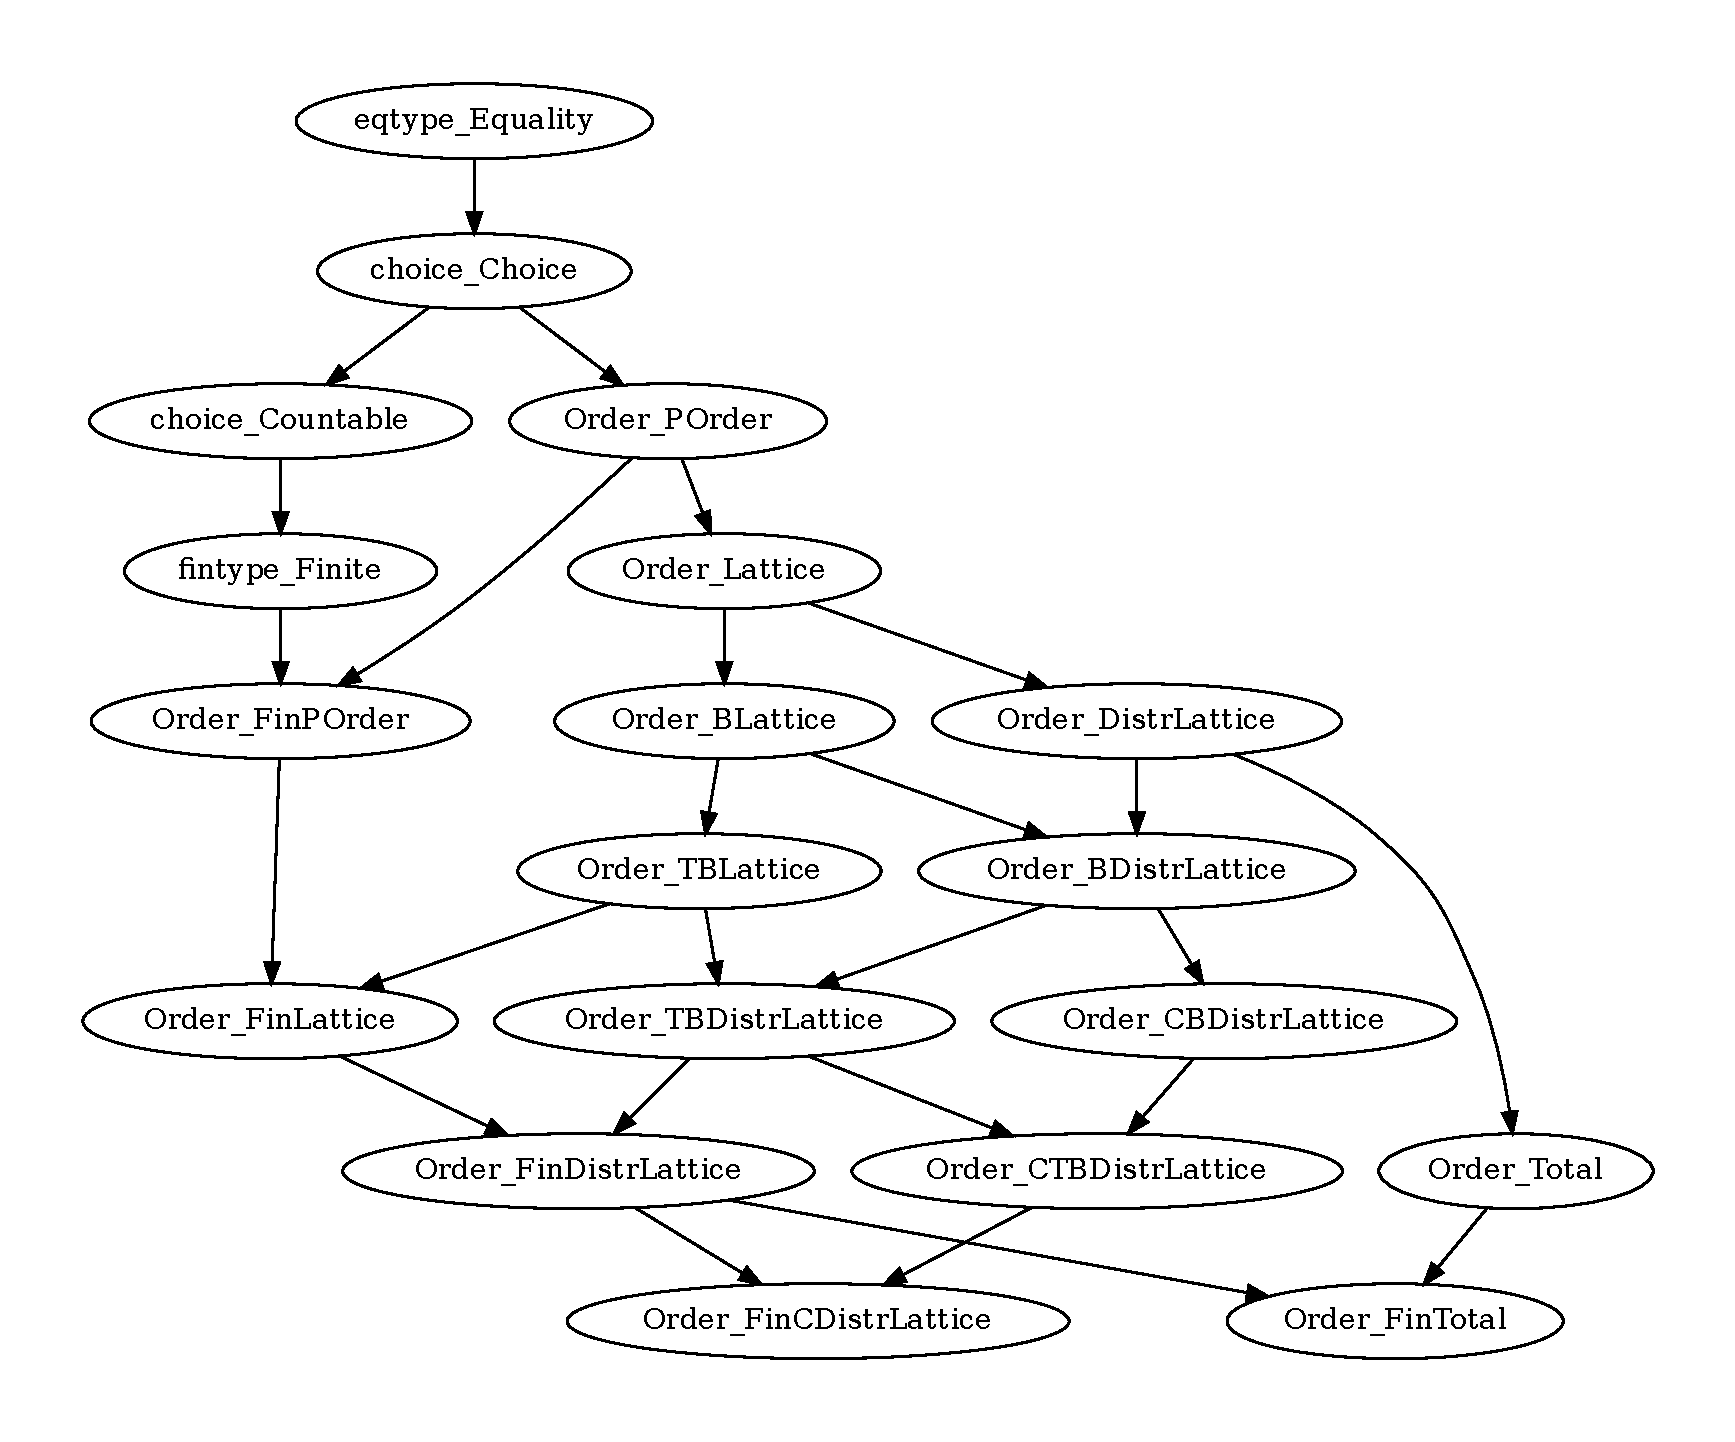
\includegraphics[width=.40\textwidth]{order.pdf}
  \caption{\small Hierarchy in order.v}
	\label{fig:order}
  \vspace{-3em}
\end{wrapfigure}
The porting consisted in declaring all the interfaces and their instances
using the new commands, \emph{without changing proofs} in any substantial way.
At the time of writing the patch~\footnote{\url{https://github.com/math-comp/math-comp/pull/733}}
amounts to about 5K lines being edited, and 5K lines being simply \emph{removed}.\\

\section{Report}

\paragraph{Documentation}

Hb is a young tool, some doc was missing, in particular how to use it
proficiently. Wiki page TODO.

MC files have an header gathering the interface the user is supposed to used.
They had to be updated, still in process. Thanks to the fact that HB has an
internal representation of the hierarchy we could provide a command to
generate a dot presentation of it, see~\ref{fig:order} for the excerpt for the
order component, which lost 1300 lines in the process. In addition to that about command to get HB
specific info.

\begin{wrapfigure}[12]{r}{.40\textwidth}
\vspace{-1em}
\begin{Verbatim}[fontsize=\footnotesize]
 HB: Order.Total.type is a structure
     (from "./ssreflect/order.v", line 1588)
 HB: Order.Total.type characterizing operations
     and axioms are:
     - le_total
 ...
 HB: Order.Total inherits from:
     - eqtype.Equality
     - choice.Choice
     - Order.POrder
     - Order.Lattice
     - Order.DistrLattice
 HB: Order.Total is inherited by:
     - Order.FinTotal
\end{Verbatim}
\vspace{-1.5em}
\caption{\small HB.about Total.}
\label{fig:orderabout}
\end{wrapfigure}

\paragraph{Performance}

TT lacks a notion af abstraction barrier. The library is already built
as if one was there, you define a concept, prove some properties, and never
unfold that concept. Still this is just a common practice with no correspondence
in TT nor in Coq vernacular. MC always suffered from per issues, concepts pile up,
and the conversion checking (term comparison) algorithm can get lost. The
library employed various locking mechanisms to mitigate the problem. HB.lock
provides one a little cost, example.
Since HB uses a more regular, but less ``efficient'' representation of classes
we had to lock a bit more. Given the library is already built with this in mind,
the changes needed (unlocking) were minimal.

\paragraph{Instances}

HB provides a built in concept of factory, a virtual interface which is
compiled to real interfaces automatically. They are mandatory to get backward
compatibility when a library evolves. However, sometimes, defining a factory is
slightly too heavy and we prefer to rely on either one or a combination of the
following techniques: either we use lemma or definition which produces a
factory from some input, or we declare an alias (identity definition) which
carries additional instances, (e.g. \verb+can_type+, \verb+sub_type+, ...) in
combination with \verb+Structure.copy T alias+ which copies all the structure
of an alias \verb+alias+ on \verb+T+.

\paragraph{Limitations}

The only part of the hierarchy we did not manage to port so far is the
interdependency between normed $\mathbb{Z}$-modules and numeric domains.
Indeed, a normed $\mathbb{Z}$-module is a $\mathbb{Z}$-module on $R$
equipped with a norm with values in a numeric domain $R$,
while a numeric domain is a $\mathbb{Z}$-module on itself, and this apparent
cyclicity which was encodable by hand is not supported by HB.
Since these structures are only really needed in MC analysis,
we managed to port MC by oversimplifying these structures.
We plan to extend HB to support this kind of self-reference
and enable the porting of MC analysis.

\paragraph{Porting activity}

One of the challenges of the porting activity was to contribute simultaneously
to several files within MC and HB with minimal bureaucracy, and making sure
everyone uses the same versions of every single dependency.

Part of this objective was achieved through a rational use of several
communication tools: a Zulip chat and a video meeting for each
collaborative dev sessions. Help from others was obtained very fast.

The other part was achieved through a nix shell which was kept updated
at all times to reflect the current reference configuration.
Anyone using this nix-shell had the guarantee to be in sync with our CI
and hence with others.

\section{Plan for Mathematical Components version 2.0}

Given MC is widely used in the community, we plan to continue releasing 1.x
releases for a while. When the first 2.x release is ready, we plan to will
keep maintaining 1.x minimally (anything that can be backported without changing the hierarchy).

\label{sect:bib}
\bibliographystyle{plain}
%\bibliographystyle{alpha}
%\bibliographystyle{unsrt}
%\bibliographystyle{abbrv}
\bibliography{bib}

%------------------------------------------------------------------------------


\end{document}

